\item A small body \( A \) starts sliding off the top of a smooth sphere of radius \( R \). Find the angle \( \theta \) (Fig. 1.25) corresponding to the point at which the body breaks off the sphere, as well as the break-off velocity of the body.
    \begin{center}
        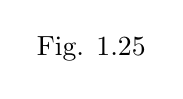
\begin{tikzpicture}
            \node at (0, 0) {Fig. 1.25};
        \end{tikzpicture}
    \end{center}